\documentclass[titlepage, a4paper, 12pt]{article}
\usepackage[english]{babel}
\usepackage[a4paper, margin=2.5cm]{geometry}
\usepackage[utf8]{inputenc}
\usepackage[T1]{fontenc}
\usepackage{graphicx}
\usepackage{verbatim}

\usepackage{amsmath, amsthm, amssymb}
\usepackage[textsize=small, textwidth=2cm]{todonotes}
\usepackage{thmtools}
\usepackage[colorlinks=true, citecolor=red]{hyperref}
\usepackage{cleveref}

\declaretheorem[name=Théorème, numberwithin=section]{theorem}
\declaretheorem[name=Lemme, sibling=theorem]{lemma}
\declaretheorem[name=Proposition, sibling=theorem]{prop}
\declaretheorem[name=Conjecture, sibling=theorem]{conjecture}


\geometry{hmargin=2.5cm, vmargin=1.5cm}
\graphicspath{ {./images/} }

\newenvironment{clem}[1]{\textcolor{purple}{Clément:~#1}}{}
\newenvironment{lumen}[1]{\textcolor{yellow}{Lumen:~#1}}{}

\let\le\leqslant
\let\ge\geqslant
\let\leq\leqslant
\let\geq\geqslant
\let\nleq\nleqslant
\let\ngeq\ngeqslant


\title{Le réveil des robots: étude sur le pire temps de réveil possible}
\date{\today}
\author{Léo Frémery \and Cyril Gavoille \and Clément legrand-duchesne}
%il faut préciser le LaBRI mais je sais pas faire

\begin{document}

	\maketitle
	
	\tableofcontents
	
	\newpage
	
	\section{Introduction}

\subsection{Présentation du problème}

Le problème du réveil des robots consiste en un robot éveillé et des robots endormis dans un disque autour de lui. Un robot éveillé peut aller vers d'autres robots pour les réveiller et l'objectif est de réveiller tous les robots le plus vite possible.

\begin{figure}[h!]
  \centering
  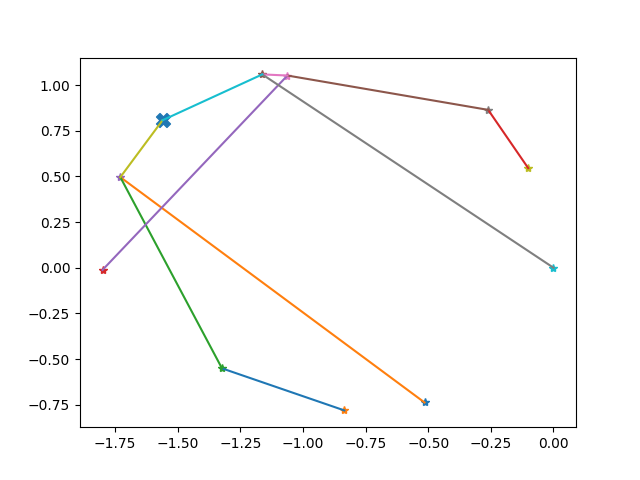
\includegraphics[scale=0.4]{opt_non_plan}
  \caption{Mon titre}
  \label{fig:opt_non_plan}
\end{figure}
\todo[inline,backgroundcolor=purple]{Il faudrait mettre les figures dans des environnements
  comme ci dessus et les référencer ainsi: Figure~\ref{fig:opt_non_plan}}

Dans le cas général, où les robots endormis sont disposés n'importe comment, le problème est NP-dur. Le meilleur algorithme existant, traçant le chemin des robots pour résoudre le cas général consiste en une programmation dynamique avec une complexité de $\frac{3^n}{\sqrt{n}}$ où $n$ est le nombre de robots.

Il reste cependant beaucoup de choses à explorer sur ce problème lorsque l'on considère des sous catégories du problème. Dans ce rapport, nous discuterons principalement de la pire configuration possible pour $n$ robots endormis soit la configuration qui crée le temps de réveil le plus grand. Le temps de réveil en question est appelé $\alpha_n$. On démontrera en particulier que $\alpha_5 < 3.603564775 < \alpha_4$ et on cassera des conjectures.

\subsection{Formalisation}

\subsubsection{problème du réveil des robots}

Le problème se place sur un plan muni de la distance euclidienne. Le robot réveillé est en $(0,0)$ et le problème se constitue donc de $n$ points chacun représentant les robots endormis dans le disque de rayon 1 et de centre $(0,0)$. On représente une solution au problème du réveil des robots par un arbre binaire couvrant tous les sommets. En effet, en chaque sommet, un robot entre, et on a alors 2 robots à déplacer si no le souhaite, formant alors un arbre binaire dont la racine est le premier robot éveillé.

On pondère les arêtes de notre arbre par la distance de l'arête et on considère la profondeur de l'arbre comme étant la somme des poids des arêtes depuis la racine. Dès lors, le temps de réveil d'un arbre donné est la longueur de la plus grande branche et le temps de réveil du problème est $min_{T} tr(T, x_1, .., x_n)$ où $tr$ est le temps de réveil sachant un arbre T et l'objectif d'un algorithme est d'obtenir un arbre minimum.

On peut alors définir $\alpha_n = max_{x_1, .., x_n} min_T tr(T, x_1, .., x_n)$

On a déjà $\alpha_1 = 1$,$\alpha_2 = \alpha_3 = 3$ et $\alpha_4 = 1 + 2\sqrt{2}$. De plus, grâce à des cônes, nous avons que $\alpha_n \leq 3 + \frac{8\pi}{\sqrt{n}}$ il est possible de faire mieux en pratique mais le résultat possède une constante plus compliquée que $8\pi$

\begin{theorem}
	Réveiller tous les robots dans un cône d'angle $\theta$ et de rayon $r$ peut être fait en un temps $\leq r(1 + chord(theta))$
\end{theorem}

	\section{Alpha 5}

Dans cette section, nous montrerons le résultat suivant, obtenu pendant mon stage avec Cyril Gavoille.

\begin{theorem}\label{alpha5borne}

$$\alpha_5 < 3.603564775$$

\end{theorem}

Dans la suite on appellera $P$ l'ensemble des points représentant les robots endormis et on considérera $\gamma$ la fonction qui à un ensemble de points associe le temps de réveil du problème associé. Pour cela, on prouvera le résultat suivant.

\begin{lemma}\label{chord}
Pour tout $P$ de taille 5, pour tout $\alpha \in \left]0, \frac{\pi}{2}\right[$, on a
$$\gamma(P) \leq \max\left(3 + \chord\left(\alpha\right), 1 + 2\chord\left(\frac{\pi}{2} - \frac{\alpha}{4}\right)\right)$$
où $\chord$ représente la longueur d'un arc de cercle de rayon 1 et d'angle $\theta$. On a donc $\chord(\theta) = 2\sin(\theta/2)$
\end{lemma}

\begin{proof}[Preuve de \ref{alpha5borne} en supposant Lemme \ref{chord}]

$\alpha \mapsto 3+\chord(\alpha)$ étant croissante $\alpha \mapsto 1 +
2\chord(\frac{\pi}{2} - \frac{\alpha}{4})$ étant décroissante, le minimum des
deux fonctions est atteint en leur croisement qui se produit pour un angle
$\alpha \approx 0.6131233066$ et dont la valeur exacte n'est pas facilement calculable. Ainsi on a

\(\forall P, \gamma(P) < 3.603564775\)

Ce qui montre que $\alpha_5 < 3.603564775$

\end{proof}

\begin{lemma}\label{worstchord}
Pour tout $n$ et $x_1$, $x_2$, ..., $x_n$ des points sur un arc de demi-cercle dans l'ordre. Alors le chemin $x_1$ - $x_2$ - ... - $x_n$ est le plus long lorsque les points sont uniformément répartis sur l' arc de demi-cercle.
\end{lemma}
\begin{proof}
On commence par identifier les points par l'angle qui les sépare d'une des deux extrémités, obtenant ainsi une suite $\left(\theta_k\right)$ identifiant nos points. Dès lors, la longueur du chemin est:

$$2\sum_{k=1}^{n-1} \sin\left(\frac{\theta_{k+1} - \theta_k}{2}\right)$$

Or $\frac{\theta_{k+1} - \theta_k}{2} \in ]0, \frac{\pi}{2}[$

Nous sommes donc sur un intervalle où $\sin$ est concave. Ainsi égaliser les $\frac{\theta_{k+1} - \theta_k}{2}$ conduit à la somme maximale et donc la longueur maximale du chemin. 
Cela implique alors que la distance entre tous les points est la même et vu qu'il est toujours préférable d'avoir des points aux extremités, on a donc que le pire cas est d'avoir les points uniformément répartis sur l'arc de demi-cercle.

\end{proof}

Dans la suite, on utilisera la notation $\gamma(T, P)$ pour donner le temps de réveil de P suivant l'arbre de réveil T.
On a alors $\forall P, \gamma(P) = \min_T(\gamma(T,P))$
et donc $\forall P, \forall T, \gamma(P) \leq \gamma(T, P)$

La preuve fonctionne en trouvant pour chaque cas un arbre dont la longueur est au pire plus petite ou égale à la borne souhaitée. La première disjonction de cas se fera sur le nombre de points constituant l'enveloppe convexe de la figure.

\subsection{Enveloppe convexe de taille 5}\label{conv5}

Soit $\alpha > 0$ et $P$ un ensemble de 5 points.

\begin{lemma}\label{conealphachord}
Supposons d'abord qu'il existe deux points inclus dans un cône d'angle $\alpha$

Dans ce cas, en réveillant les deux robots dans le cône avec celui initial, on peut aller réveiller les trois derniers où qu'ils soient dans le cercle. Réveiller les robots dans un cône d'angle $\alpha$ prend au plus un temps $1 + \chord(\alpha)$.
On peut donc utiliser \cref{coneworst} pour réveiller tout le monde avec $\gamma(P) \leq 1 + \chord(\alpha) + 2 = 3 + \chord(\alpha)$
\end{lemma}

Par la suite on tournera notre figure en sélectionnant un point tel que son axe coupe le cercle en deux demi-cercles contenant chacun 2 points. Un tel point existe toujours. En effet, si l'on prend un point au hasard, si la répartition est 4-0  alors le deuxième voisin (du coté où il y a le plus de point) a une répartition 2-2. Si la répartition est 3-1 alors on peut tourner notre axe du côté où il y a les 3 points jusqu'à croiser un point. Si le premier point que l'on trouve est du coté où il n'y avait qu'un seul point, alors il faut aller chercher le deuxième voisin comme avant qui sera en 2-2 sinon, dans le cas où le premier point rencontré est du côté des 3 points, alors le nouveau point trouvé convient. (si les deux cas sont vrais, les deux solutions fonctionnent)

\begin{figure}[h!]
 \centering
  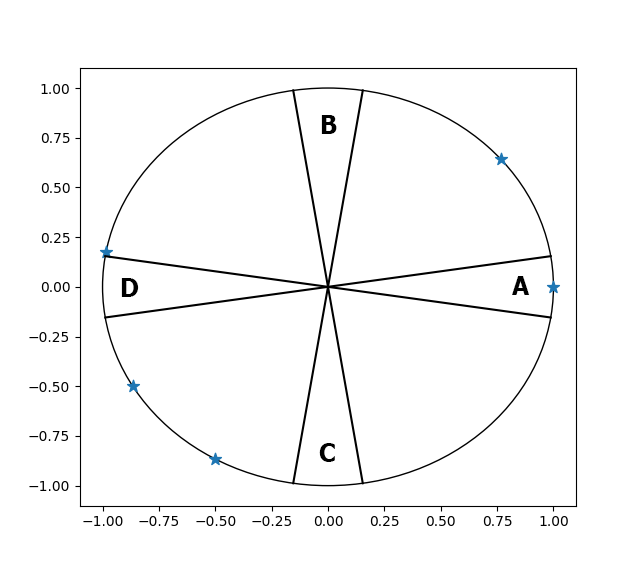
\includegraphics[scale=0.4]{initial_position}
 \caption{position initiale}
 \label{fig:initial_position}
\end{figure}

  On sépare ensuite le cercle en différents cônes d'angle $\alpha$ nommés $A$,
  $B$, $C$, et $D$ comme sur la Figure \ref{fig:initial_position}. C'est en
  effet ce $\alpha$ qui apparaîtra dans la formule finale. On notera $|X|$ le
  nombre de point dans le cône $X$.

\subsection*{Description des Cas}

\begin{itemize}
	\item \ref{1cas} $\exists X \in {A,B,C,D}, |X| > 1$
	\item \ref{2cas} $|D| = 0$
	\item \ref{3cas} $|B| = |C| = 0$ (et $|D| = |A| = 1$)
	sans perte de généralité, on suppose que le point de $D$ appartient au demi-cercle du haut
	\begin{itemize}
		\item \ref{3cas1} le deuxième point du haut est entre $A$ et $B$
		il reste à décider de la position des points du bas
		\begin{itemize}
			\item \ref{3cas11} 1 point du bas entre $A$ et $C$ ainsi que le dernier entre $C$ et $D$.
			\item \ref{3cas12} 2 points entre $C$ et $D$
			\item \ref{3cas13} 2 points entre $A$ et $C$
		\end{itemize}
		\item \ref{3cas2} le deuxième point du haut est entre $B$ et $D$
		de même il reste à décider de la position des points du bas
		\begin{itemize}
			\item \ref{3cas21} 2 points entre $A$ et $C$
			\item \ref{3cas22} 2 points entre $C$ et $D$
			\item \ref{3cas23} 1 point dans chacune des deux zones
		\end{itemize}
	\end{itemize}
	\item \ref{4cas} $|A| = |B| = |C| = |D| = 1$
	\begin{itemize}
		\item \ref{4cas1} si le 5 ème point est dans un cône diagonal d'angle $\alpha$
		\item \ref{4cas2} sinon
	\end{itemize}
	\item \ref{5cas} $|A| = |D| = 1$, $|C| = 0$ et $|D| = 1$
		par symétrie, le cas $|C| = 1$, $|D| = 0$ rentre aussi dans cette catégorie, concluant la disjonction présente
	\begin{itemize}
		\item \ref{5cas1} le point dans $D$ appartient au demi-cercle du haut
		\begin{itemize}
			\item \ref{5cas11} si on a en bas un point de chaque côté
			\item \ref{5cas12} si les deux point du bas sont entre $C$ et $D$
			\item \ref{5cas13} si les deux points du bas sont entre $A$ et $C$
		\end{itemize}
		\item \ref{5cas2} le point dans $D$ appartient au demi-cercle du bas
		on a donc 4 cas selon le positionnement du point en haut et en bas
		\begin{itemize}
			\item \ref{5cas21} Point du haut entre $A$ et $B$ et point du bas entre $A$ et $C$
			\item \ref{5cas22} Point du haut entre $A$ et $B$ et point du bas entre $C$ et $D$
			\item \ref{5cas23} Point du haut entre $B$ et $D$ et point du bas entre $C$ et $D$
			\item \ref{5cas24} Point du haut entre $B$ et $D$ et point du bas entre $A$ et $C$
		\end{itemize}
	\end{itemize}
\end{itemize}

\subsection*{1er cas}\label{1cas} $\exists X \in {A,B,C,D}, |X| > 1$

Alors, il existe deux points dans un cône d'angle $\alpha$. On peut donc appliquer le Lemme \ref{conealphachord} pour conclure

\subsubsection*{2ème cas}\label{2cas} $|D| = 0$

On prend $T$ l'arbre commençant au noeud de $A$ et explorant de part et d'autre
de son axe en commençant par le noeud le plus proche (voir Figure \ref{fig:2eme_cas}).
Soit $P'$ l'ensemble de point sur le cercle où les deux points des demi-cercles sont répartis entre $A$ et $D$.
On a $\gamma\left(P\right) \leq  \gamma\left(T, P\right) \leq \gamma\left(T, P'\right)$

\begin{figure}[h!]
  \centering
  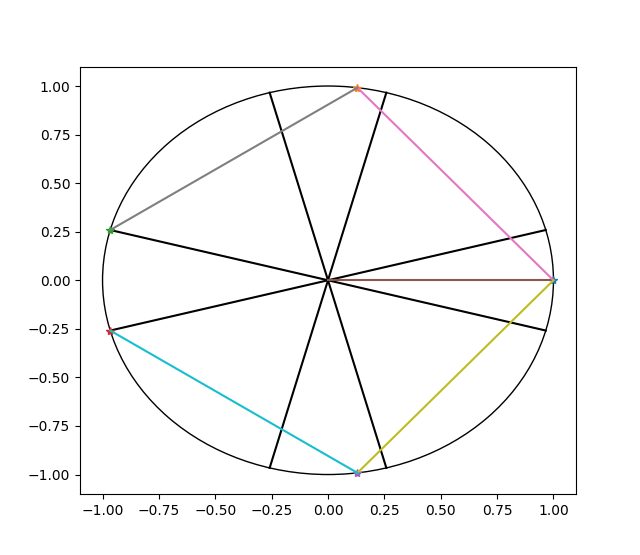
\includegraphics[scale=0.4]{2eme_cas}
  \caption{Résolution 2e cas}
  \label{fig:2eme_cas}
\end{figure}

En effet, d'après le \cref{worstchord}, le pire cas pour $P$ est d'avoir un point le plus loin possible de A et d'avoir des arcs égaux, positionnant donc le dernier point du demi-cercle pile entre le point de $A$ et celui collant $D$. On a alors
$$\gamma\left(P\right) \leq \gamma\left(T, P'\right) = 1 + 2\chord\left(\frac{\pi}{2} -
  \frac{\alpha}{4}\right)$$

\subsubsection*{3ème cas}\label{3cas} $|B| = |C| = 0$ ($|A| = 1$ et $|D| = 1$)
Par symétrie, on peut considérer que le point dans $D$ appartient au demi-cercle du haut et donc que l'on a un seul point en haut qui ne soit pas dans $D$ que l'on nommera $b$.

\begin{figure}[h!]
 \begin{subfigure}[t]{0.45\textwidth}
   \centering
   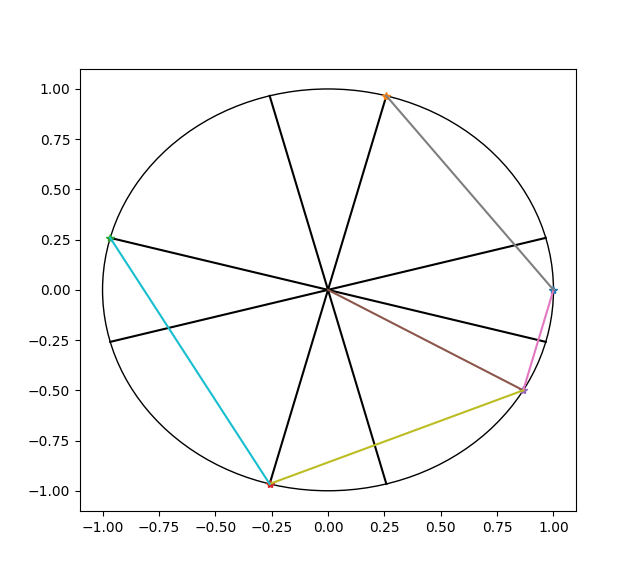
\includegraphics[scale=0.4]{3eme_cas1}
   \caption{Résolution 3e cas n1}
   \label{fig:3eme_cas1}
 \end{subfigure}
 \hfill
 \begin{subfigure}[t]{0.45\textwidth}
   \centering
  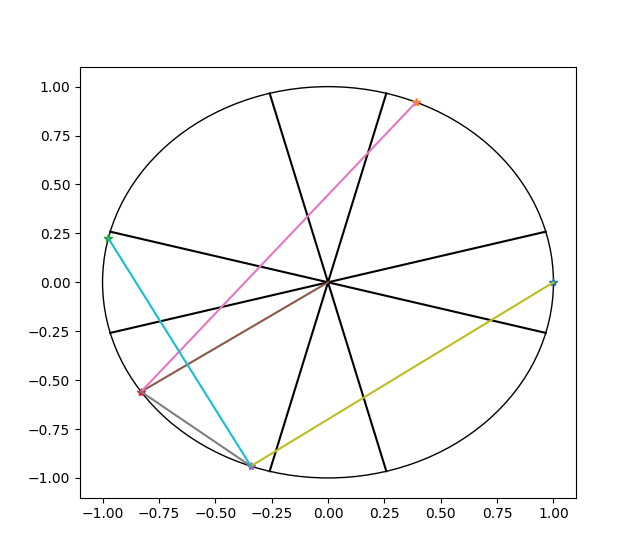
\includegraphics[scale=0.4]{3eme_cas2}
  \caption{Résolution 3e cas n2}
  \label{fig:3eme_cas2}
 \end{subfigure}
 \hfill 
 \begin{subfigure}[t]{0.45\textwidth}
   \centering
  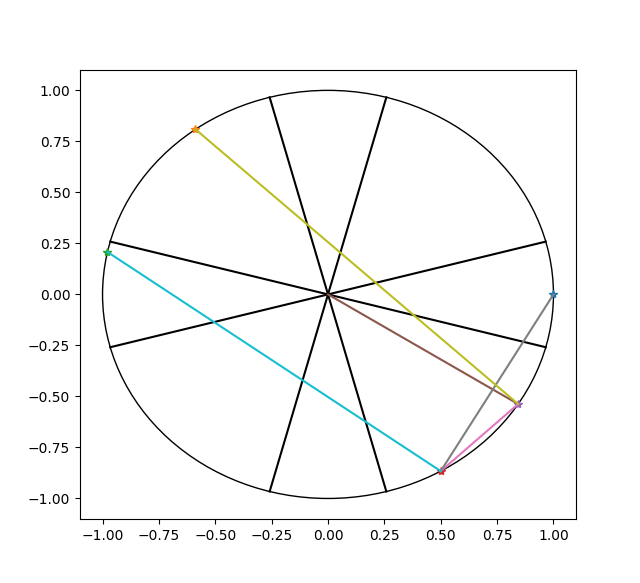
\includegraphics[scale=0.4]{3eme_cas3}
  \caption{Résolution 3e cas n3}
  \label{fig:3eme_cas3}
 \end{subfigure}  
 \hfill 
 \begin{subfigure}[t]{0.45\textwidth}
   \centering
   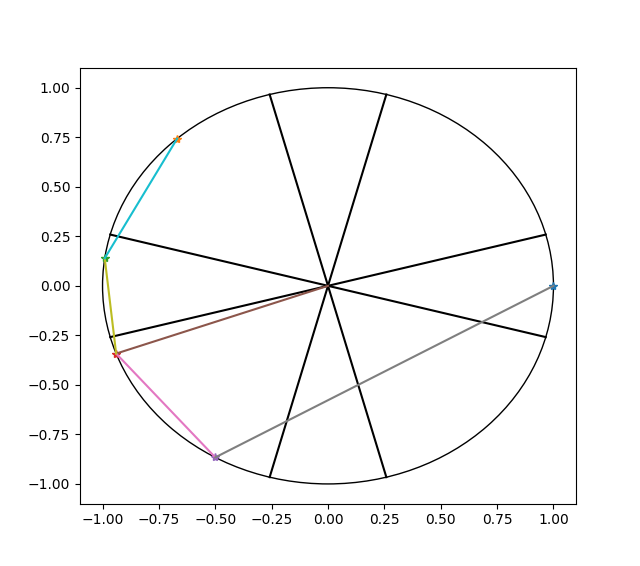
\includegraphics[scale=0.4]{3eme_cas4}
   \caption{Résolution 3e cas n4}
   \label{fig:3eme_cas4}
 \end{subfigure}
 \hfill
 \begin{subfigure}[t]{0.45\textwidth}
   \centering
   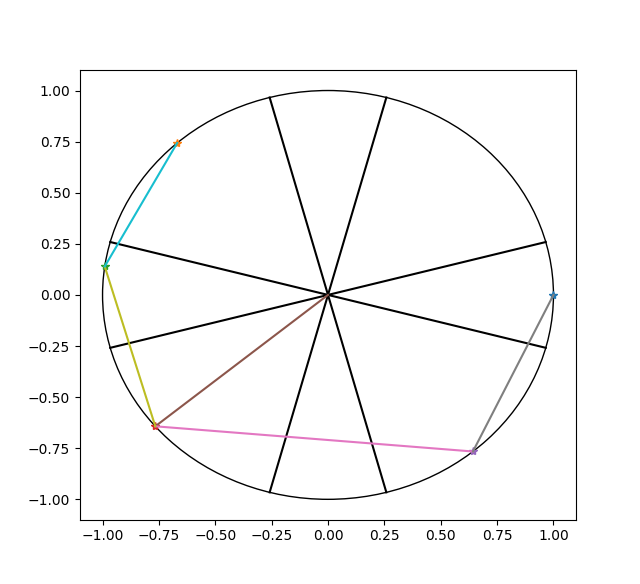
\includegraphics[scale=0.4]{3eme_cas5}
   \caption{Résolution 3e cas n5}
   \label{fig:3eme_cas5}
 \end{subfigure}
 \caption{Résolutions du 3e cas ($|B| = |C| = 0$ et $|A| = |D| = 1$)}
\end{figure}

\begin{itemize}

\item \label{3cas1} Si $b$ est entre $A$ et $B$.

\begin{itemize}

\item \label{3cas11} Si $b$ entre $A$ et $B$ et il y a en bas 1 point de chaque
  côté de $C$.

On choisit pour $T$ l'arbre commençant en bas à gauche et séparant le travail
des robots en 2 comme avant (voir Figure~\ref{fig:3eme_cas1}).
On prend ensuite le pire cas possible pour ce $T$.

%\begin{figure}[h!]
%  \centering
% 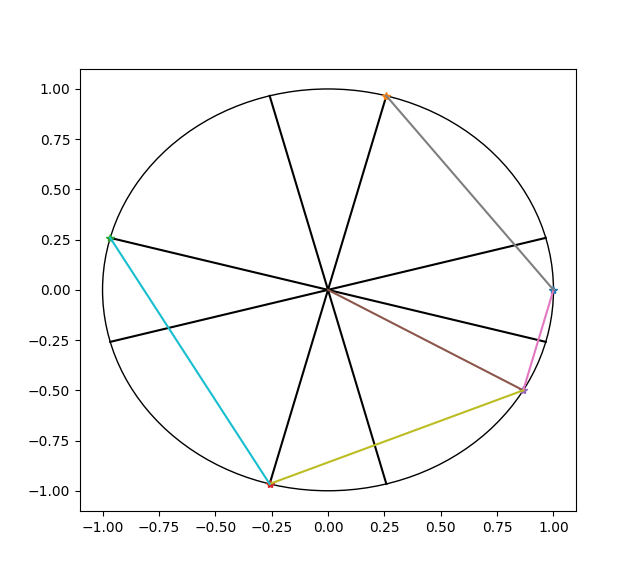
\includegraphics[scale=0.4]{3eme_cas1}
%  \caption{Résolution 3e cas n1}
%  \label{fig:3eme_cas1}
%\end{figure}

En oubliant pas que grâce au \cref{conealphachord} l'angle entre $a$ et le point en bas à gauche est d'au moins $\alpha$ on peut donc appliquer le Lemme \ref{worstchord} afin de conclure
$\gamma(P) \leq 1 + 2\chord(\frac{\pi}{2} - \frac{\alpha}{4})$\todo[inline,backgroundcolor=red]{Cela
  rejoint mon commentaire dans le premier cas: ce qui est utilisé ici est que
  l'écart entre les points est d'au moins $\alpha$., ce qui est plus fort que
  ``aucun des cônes $A$,.. $D$ ne contient deux points''}

\item \label{3cas12} Si $b$ entre $A$ et $B$ et deux points entre $C$ et $D$,
	Considérons $T$ l'arbre représenté Figure~\ref{fig:3eme_cas2}.

%\begin{figure}[h!]
%  \centering
%  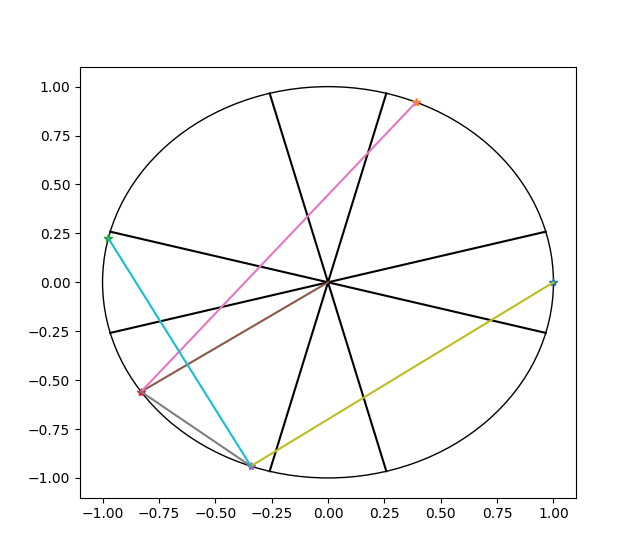
\includegraphics[scale=0.4]{3eme_cas2}
%  \caption{Résolution 3e cas n2}
%  \label{fig:3eme_cas2}
%\end{figure}

Ici on néglige la branche menant à b car elle a une longueur totale d'au plus 3 (ce sera
aussi fait dans les cas suivants).
La longueur de la branche bleue est ici majorée par $1+\chord\left(\frac{\pi}{2} - \alpha\right)+\chord(\frac{\pi}{2}) \leq 1 + 2\chord(\frac{\pi}{2} - \frac{\alpha}{4})$.
Et pour la dernière branche, on applique le \cref{worstchord} pour obtenir
cette borne exacte

$$\gamma(P) \leq 1 + 2\chord\left(\frac{\pi}{2} -
  \frac{\alpha}{4}\right)$$

\item \label{3cas13} Si $b$ est entre $A$ et $B$ et deux points entre $A$
  et $C$ on applique le même arbre. En effet, la seule différence avec le cas d'avant est l'emplacement du point intermédiaire du bas. Or \cref{worstchord} n'est pas impacté par la position particulière de ce point. Le résultat est donc préservé.
  
\end{itemize}

\item \label{3cas2} Si $b$ est entre $C$ et $D$.

\begin{itemize}

\item \label{3cas21} Le seul cas difficile est celui où les deux points du bas sont entre $A$ et $C$.
\st{suivant l'arbre suivant:} \add{Considérons $T$ l'arbre représenté Figure~\ref{fig:3eme_cas3}.}
%\begin{figure}[h!]
%  \centering
  % 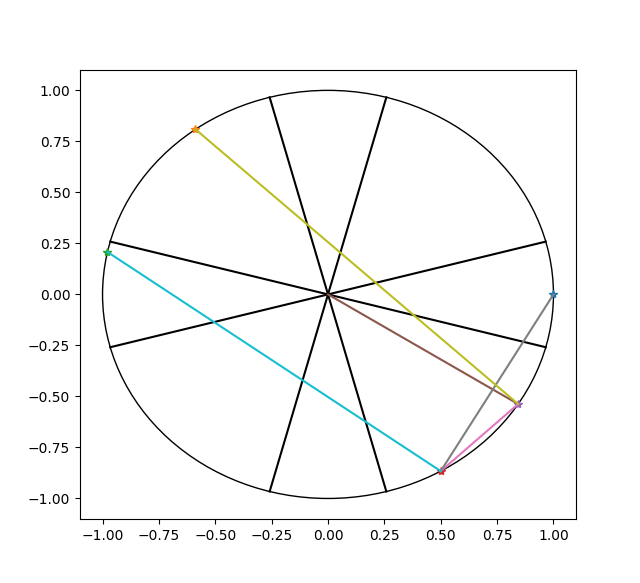
\includegraphics[scale=0.4]{3eme_cas3}
%  \caption{Résolution 3e cas n3}
%  \label{fig:3eme_cas3}
%\end{figure}

La branche bleue ici se résout encore une fois par \ref{worstchord}
La branche jaune est négligée
et la branche violette permet le calcul de son pire cas en maximisant la longueur des cordes en respectant les contraintes angulaires. (en particulier que l'angle entre deux points doit être d'au moins $\alpha$)

on obtient alors
\begin{align*}
\gamma(P) &\leq \max\left(1+2\chord\left(\frac{\pi}{2} - \frac{\alpha}{4}\right), 1 + \chord\left(\frac{\pi}{2} - \frac{3\alpha}{2}\right) + \chord\left(\frac{\pi}{2} - \frac{\alpha}{2}\right)\right) \\
&\leq 1+2\chord\left(\frac{\pi}{2} - \frac{\alpha}{4}\right)
\end{align*}

\item \label{3cas22} Si l'on a 2 points entre $C$ et $D$, alors on peut
  effectuer l'arbre \add{représenté Figure~\ref{fig:3eme_cas4}.}
%\begin{figure}[h!]
%  \centering
%  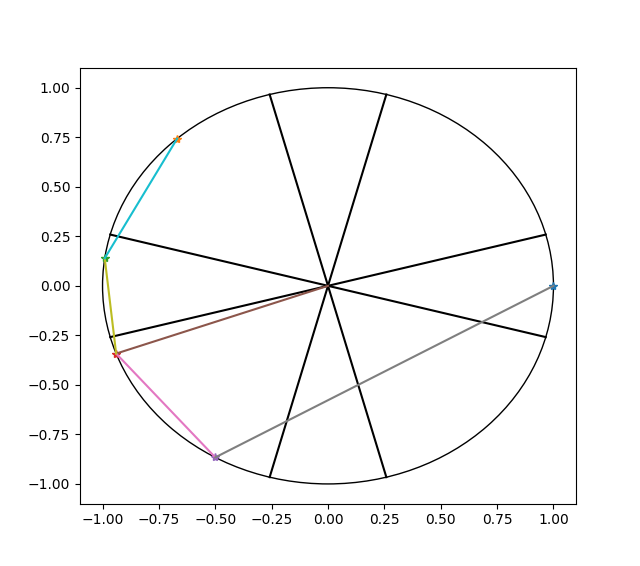
\includegraphics[scale=0.4]{3eme_cas4}
%  \caption{Résolution 3e cas n4}
%  \label{fig:3eme_cas4}
%\end{figure}

On peut alors comme d'habitude utiliser le \cref{worstchord} pour conclure

\item \label{3cas23} Pour dernier cas, nous avons 1 point de part et d'autre de
  la vertical en bas alors par un chemin similaire au point précédent \add{(voir
    Figure~\ref{fig:3eme_cas5}).}

% \begin{figure}[h!]
%   \centering
%   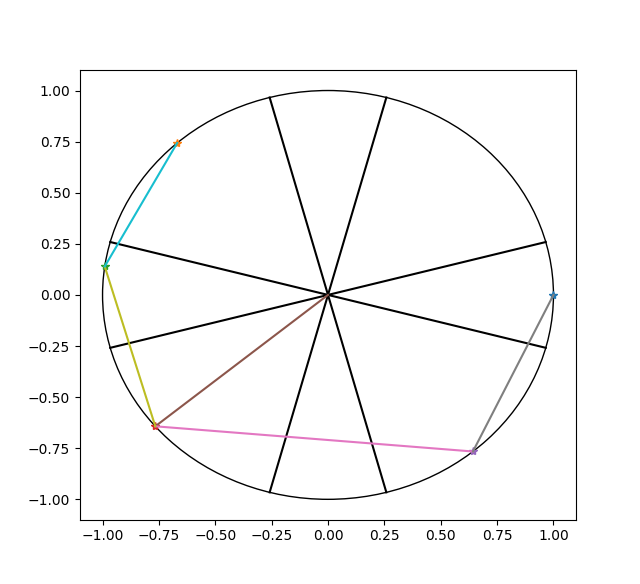
\includegraphics[scale=0.4]{3eme_cas5}
%   \caption{Résolution 3e cas n5}
%   \label{fig:3eme_cas5}
% \end{figure}

Comme la dernière fois le \cref{worstchord} nous permet de conclure

\end{itemize}
\end{itemize}

\subsubsection*{4eme cas}\label{4cas} $|A| = |B| = |C| = |D| = 1$

il reste donc un 5eme point à placer qui se trouve dans un des cônes diagonaux.

\begin{itemize}

\item \label{4cas1} si il est dans un cône d'angle $\alpha$ au centre du cône diagonal.

on a alors le chemin standard commençant par le 5ème point qui nous donne par le \cref{worstchord}: $\gamma(P) \leq 1 + 2\chord(\frac{\pi}{2} - \frac{\alpha}{4})$

\item \label{4cas2} si ca n'est pas le cas alors on prend l'arbre commençant en ce 5 ème point mais allant vers le point le plus proche et le plus éloigné ainsi

%\begin{figure}[h!]
%  \centering
  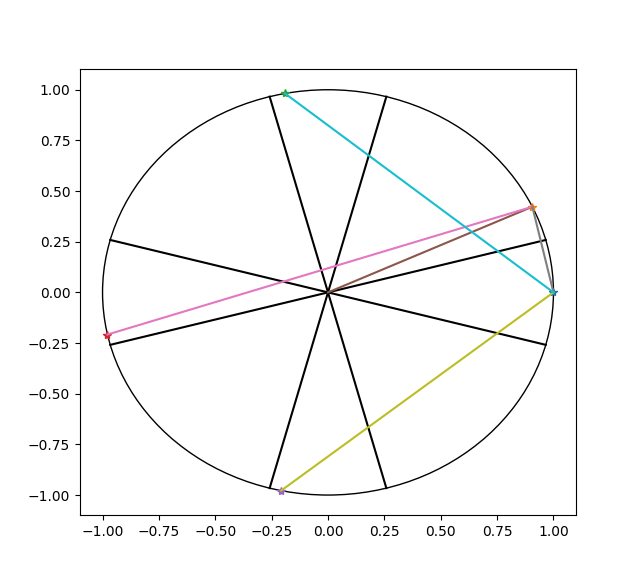
\includegraphics[scale=0.4]{4eme_cas}
%  \caption{Résolution 4e cas}
%  \label{fig:4eme_cas}
%\end{figure}

La branche rose est négligée
la branche bleue est a sa première partie bornée par une corde de taille $\frac{\pi}{4}$ car le point du milieu est en dessous de la ligne diagonal d'un angle au moins $\frac{\alpha}{2}$ et la deuxième partie par $\frac{\pi}{2} + \alpha$
la branche jaune est symétrique à la branche bleue.

on a donc $\gamma(P) \leq 1 + \chord(\frac{\pi}{4}) + \chord(\frac{\pi}{2} + \alpha) \leq \max(3 + \chord(\alpha), 1 + 2\chord(\frac{\pi}{2} - \frac{\alpha}{4}))$

\end{itemize}

\subsubsection*{5ème cas}\label{5cas} $|B| = |A| = |D| = 1, |C| = 0$
à noter que par symétrie, ca s'applique pour $|B| = 0$ et $|C| = 1$

\begin{itemize}

\item \label{5cas1} Si le point dans D appartient au demi-cercle du haut:

\begin{itemize}

\item \label{5cas11} Si en bas il y a un point de chaque côté, on choisit le point en bas qui se trouve du côté de B et on termine de façon standard. On a alors $\gamma(P) \leq 1 + 2\chord(\frac{\pi}{2} - \frac{\alpha}{4})$

\item \label{5cas12} si en bas on a les deux points du même côté, on commence par celui au milieu des deux points qui le collent pour obtenir le même résultat.
Dans le cas où les deux points sont entre C et D on a donc

%\begin{figure}[h!]
%  \centering
  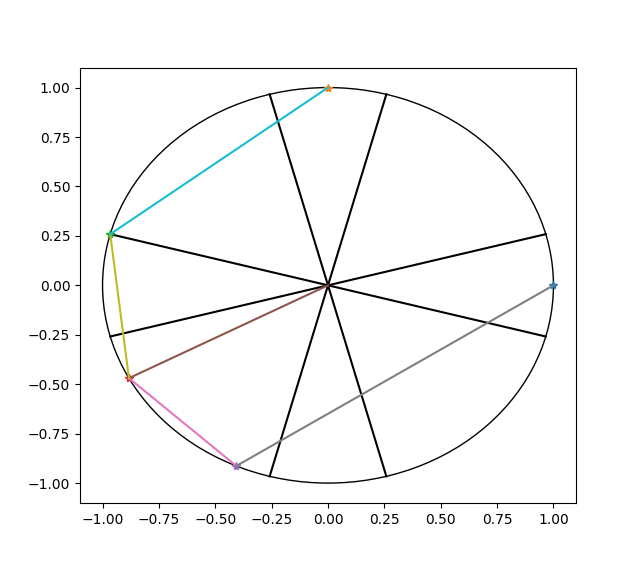
\includegraphics[scale=0.4]{5eme_cas1}
%  \caption{Résolution 5e cas n1}
%  \label{fig:5eme_cas1}
%\end{figure}

Nous sommes ici encore en capacité d'utiliser le \cref{worstchord}

\label{5cas13} Dans le cas où les deux sont entre A et C on a

%\begin{figure}[h!]
%  \centering
  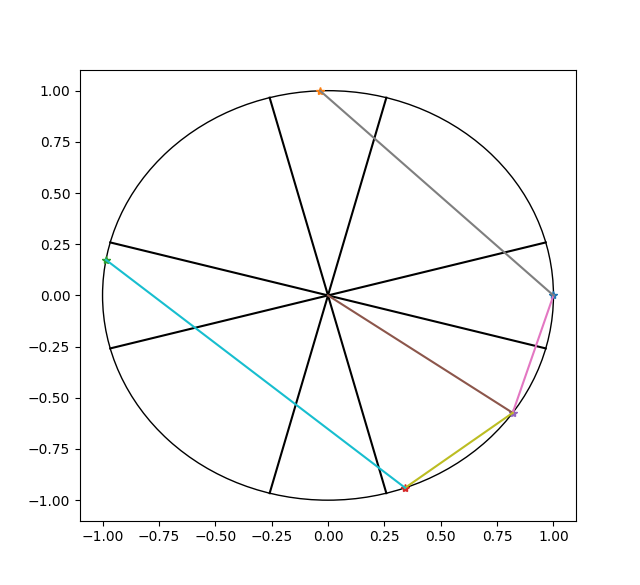
\includegraphics[scale=0.4]{5eme_cas1bis}
%  \caption{Résolution 5e cas n1bis}
%  \label{fig:5eme_cas1bis}
%\end{figure}

grâce à l'écart d'angle entre les points, on a bien encore une fois les
conditions d'applications du \cref{worstchord}

\end{itemize}

\item \label{5cas2} Si le point dans D appartient au demi-cercle du bas, on a 4 cas

\begin{itemize}

\item \label{5cas21} si point libre du haut entre A et B et point du bas entre A et C

%\begin{figure}[h!]
%  \centering
  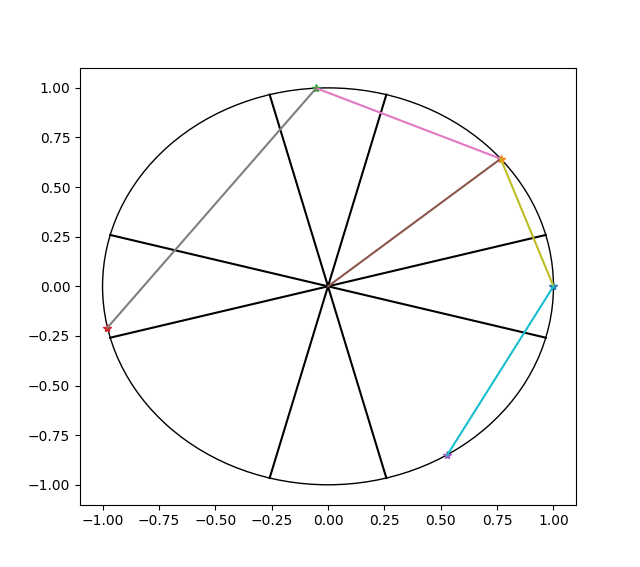
\includegraphics[scale=0.4]{5eme_cas2}
%  \caption{Résolution 5e cas n2}
%  \label{fig:5eme_cas2}
%\end{figure}

en oubliant pas que le point de départ est forcément éloigné d'un angle $\alpha$ de $a$ on a bien le résultat par le \cref{worstchord}

\item \label{5cas22} si point libre du haut entre A et B et point du bas entre C et D alors cela dépend de $b$. Si $b$ est sur le côté droit, on commence effectue cet arbre:

%\begin{figure}[h!]
%  \centering
  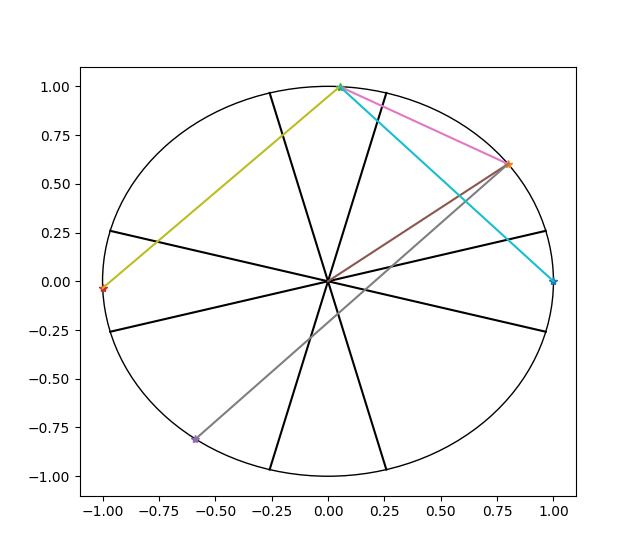
\includegraphics[scale=0.4]{5eme_cas3}
%  \caption{Résolution 5e cas n3}
%  \label{fig:5eme_cas3}
%\end{figure}

on a alors

$\gamma(P) \leq \max\left(1+2\chord\left(\frac{\pi}{2} - \frac{\alpha}{4}\right), 1 + \chord\left(\frac{\pi}{2} - \alpha\right) + \chord\left(\frac{\pi}{2}\right)\right) \leq 1+2\chord\left(\frac{\pi}{2} - \frac{\alpha}{4}\right)$

si maintenant $b$ est sur le côté gauche, on peut commencer par $b$. On effectuant un arbre classique, le côté gauche a la bonne borne et le côté droit est facile

\item \label{5cas23} si point libre du haut entre B et D et point libre du bas entre C et D on a l'arbre suivant.

%\begin{figure}[h!]
%  \centering
  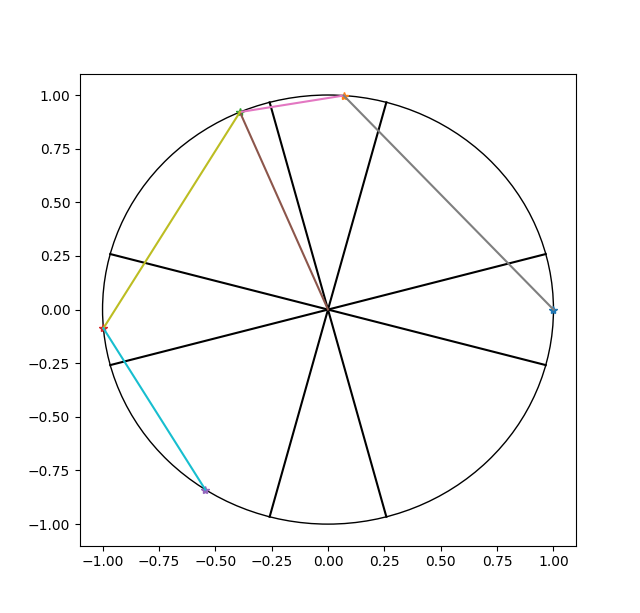
\includegraphics[scale=0.4]{5eme_cas4}
%  \caption{Résolution 5e cas n4}
%  \label{fig:5eme_cas4}
%\end{figure}

\item \label{5cas24} si point libre du haut entre B et D et point libre du bas entre A et C cela dépend à nouveau de $b$. Si $b$ à droite on a (en allant vers le point le plus proche):

%\begin{figure}[h!]
%  \centering
  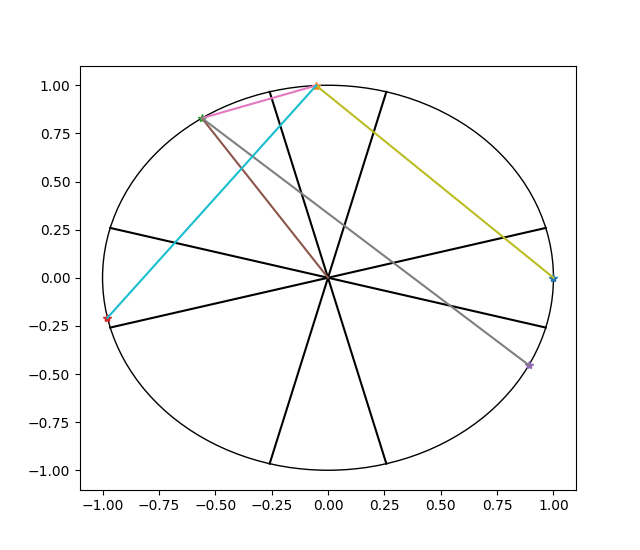
\includegraphics[scale=0.4]{5eme_cas5}
%  \caption{Résolution 5e cas n5}
%  \label{fig:5eme_cas5}
%\end{figure}

en effet, on obtient alors en allant vers le plus proche que la longueur de la branche qui effectue le croisement est plus petite que $1+\chord\left(\frac{\frac{\pi}{2} + \frac{\alpha}{2}}{2}\right) + \chord\left(\frac{\pi}{4} + \frac{\alpha}{4}\right)$ or cette valeur est inférieure à $\max\left(3 + \chord\left(\alpha\right), 1 + 2\chord\left(\frac{\pi}{2} - \frac{\alpha}{4}\right)\right)$ on a alors le résultat souhaité.

cependant si $b$ est à gauche on peut alors commencer par $b$ pour finir le problème comme la dernière fois.

\end{itemize}
\end{itemize}

\subsection{Enveloppe convexe de taille 4 ou 3}\label{conv3}

Désormais, il faut terminer avec les cas où l'enveloppe convexe est de taille 3 ou 4. Heureusement, ces cas sont plus simples.
Si l'enveloppe convexe est de taille 3, on va vers le point le plus proche du centre qui soit à l'intérieur de l'enveloppe convexe, ensuite un des deux robots ira chercher le deuxième point à l'intérieur tandis que le deuxième ira réveiller le point le plus proche du triangle avant d'aller sur les deux autres.

%\begin{figure}[h!]
%  \centering
  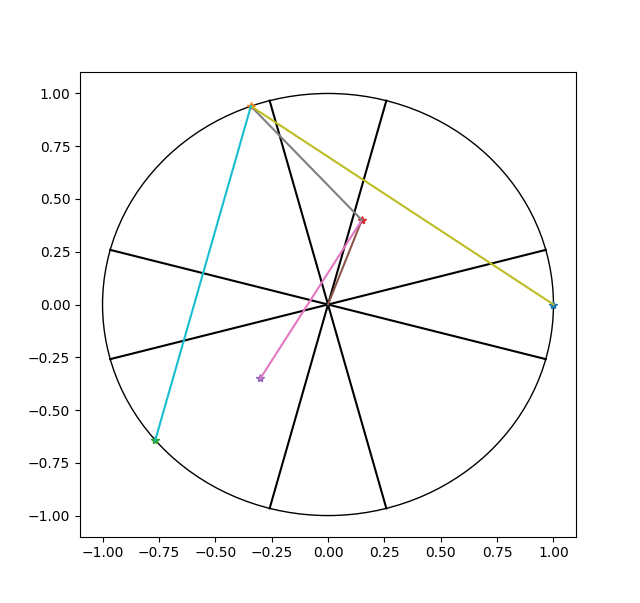
\includegraphics[scale=0.4]{n3}
%  \caption{Résolution Pour une enveloppe convexe de taille 3}
%  \label{fig:n3}
%\end{figure}

En effet, le pire cas est si le point que l'on rejoint en premier est projeté sur l'enveloppe convexe orthogonalement ce qui nous donne $\exists \theta, \gamma(P) \leq \cos(\theta) + \sin(\theta) + 2 \leq \sqrt{2} + 2 \leq \max(3 + \chord(\alpha), 1 + 2\chord(\frac{\pi}{2} - \frac{\alpha}{4}))$

Note: En réalité, cela fonctionne quelque soit l'emplacement du deuxième point à l'intérieur, et donc également si il n'est pas dans l'enveloppe connexe, et il est donc possible de traiter par exactement la même méthode le cas où l'enveloppe convexe est de taille 4.

\subsection{conclusion de la preuve}

Cela conclut la preuve, trouvant ainsi une borne pour $\alpha_5$ montrant également que $\alpha_5 < \alpha_4$. On remarquera que plus on fait de disjonctions de cas, plus il est possible d'affiner le choix de l'arbre selon les situations, permettant ainsi d'obtenir une meilleure borne.
	
	\section{Implémentation C++}

Il n'est pas clair quelle est la forme de l'ensemble de point qui mènera au pire temps de réveil. Cependant, on peut conjecturer que pour le cas pair, il s'agirait d'une répartition uniforme des points sur le cercle et c'est dans ce but que l'on a étudié selon divers algorithmes le temps de réveil du cas "uniforme" à $n$ robots que l'on appelera $\beta_n$.

En utilisant nos algorithmes afin de tracer des approximations de $\beta_n$, on a pu émettre une conjecture indiquant que $\beta_{2n}$ serait décroissante. Cela serait un pas en avant dans la recherche pour montrer que $\alpha_4$ est bien le maximum strict.

Pour tenter de s'assurer de la véracité de ces formules, il est d'abord intéressant de la tester pour divers valeurs de $n$. Mon travail a donc été ici la réimplémentation en C++ d'algorithmes python afin de les accélérer et en particulier pour le cas où les points sont répartis uniformément dans le cercle.

\subsection{Premier algorithme "Segment"}

\large{principe de l'algorithme} il se positionne sur un point de la forme convexe, et choisi un autre point qui coupera alors le polygone en deux parties, On envoi alors un robot pour chacune de ces parties qui s'occuperont récursivement de leurs propres polygones.
Il est important de noter que l'on utilise un cache pour introduire de la programmation dynamique et réduire la complexité.

Segment est un algorithme qui a été créé pour travailler sur le cas général dans l'espoir d'obtenir un bon algorithme polynomial pour le résoudre. Le problème étant NP-dur, cet algorithme ne permet en effet pas de résoudre le cas général et manque des solutions. Cyril Gavoille a tout de même prouvé qu'il existe un ordre d'entrée des points permettant à segment de donner la solution optimale. Cependant, étant donné qu'il existe $n!$ solutions, cela n'est qu'une observation.
Dans le cas Convexe, on aurait pu espérer Cependant qu'en donnant les points dans l'ordre direct on puisse obtenir une solution optimale. En effet, Le cas où les points sont en position convexe laisse une question ouverte sur son appartenance à $P$. 

il est important d'observer que dans le cas convexe avec l'ordre dans le sens des aiguilles d'une montre de la forme convexe, la solution obtenue présente des arêtes qui ne s'intersectent pas, on dit que cette solution est planaire. 

Dans le cadre d'un cercle où les points sont répartis uniformément, une optimisation excellente consiste à introduire une certaine subjectivité, un duo de robot sur un point n'aura pour environnement de travail qu'un segment défini par sa longueur à gauche et à droite de lui. Il n'existe alors que $n^2$ possibilités. On obtient alors un algorithme polynomial, rapide pour résoudre les $\beta_n$. 

Enfin, c'est ce qu'il aurait été possible de dire si segment permettait de donner les solutions optimales. Malheureusement, cela n'a pas été prouvé et dans le cas plus général convexe, on observe des solutions optimales non planaires et donc automatiquement, segment n'est pas optimal, en voici un exemple:

  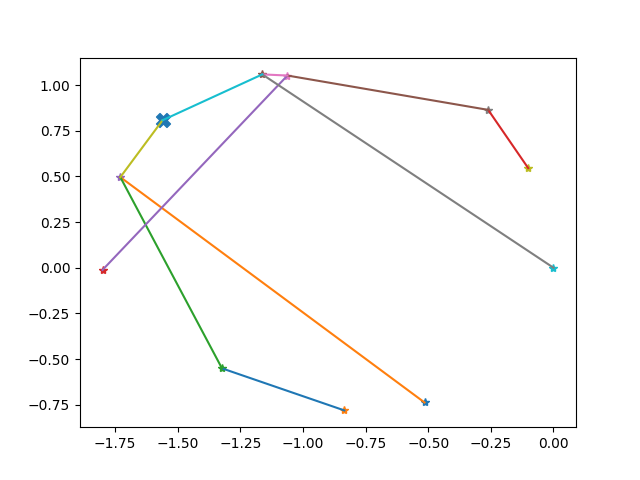
\includegraphics[scale=0.5]{opt_non_plan}
  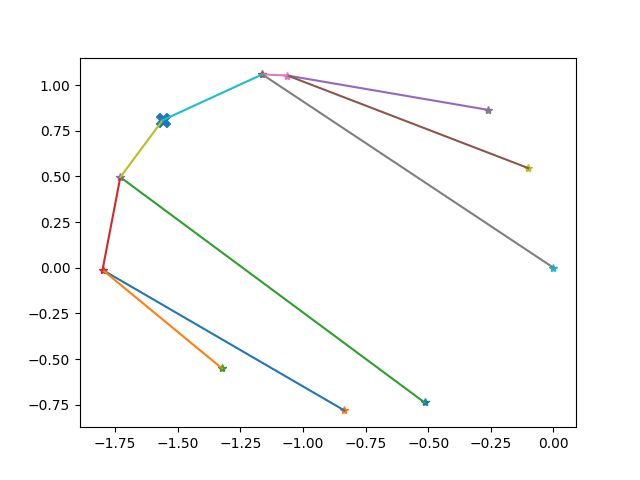
\includegraphics[scale=0.5]{seg_non_plan}\label{fig:segopt}

On a à gauche la solution optimale présentant un croisement, exploitant que la branche à gauche est plus courte que celle de droite tandis que sur l'image de droite, on trouve la meilleure solution planaire possible, soit celle donnée par segment. On voit donc bien que segment ne résout pas complètement le cas convexe mais l'approxime.

Ma contribution sur ce sujet aura été l'implémentation et l'optimisation en C++ qui aura ainsi permis d'aller explorer la position uniforme jusqu'à $n = 1000$ sans prendre trop de temps. Il reste encore ouvert si Segment du cas convexe permet de résoudre le cas uniforme et cela forme une nouvelle conjecture.

\subsection{Brute force}

Comme son nom l'indique, cet algorithme cherche à tester toutes les solutions possibles afin de trouver la meilleure possible. En utilisant un cache, il est possible de montrer que cet algorithme est dans le cas général en $\frac{3^n}{\sqrt{n}}$. Avant mon arrivée, pour calculer le temps optimal pour le cas circulaire à $n = 17$ points, il fallait à un bon ordinateur 5 minutes et 17 secondes rendant très compliqué voir impossible d'aller plus loin et donc de vérifier nos conjectures qui ne deviennent ambigües qu'à $n$ grand.

Dans l'objectif de pouvoir aller plus loin dans l'analyse des $\beta_n$. J'ai également réimplémenter l'algorithme brute force en C++ permettant alors de calculer le cas $n = 17$ en 1 minute et 18 seconde, un progrès significatif surtout que ce temps est obtenu sur un pc bien moins bon.
Ironiquement, la plus grand optimisation aura été de rajouter "-O3" à la commande de compilation pour laisser le compilateur tout optimiser à sa façon, utilisant des fonctions avancées du processeur. On descend alors à 18 secondes.
Pour que cela soit possible, que le compilateur puisse optimiser autant, il faut noter qu'une grande amélioration aura été de représenter les ensembles de points présents en grande quantité dans le code par une classe spéciale basée sur un entier 64 bit où un 1 en position i signifie que i est dans l'ensemble. Un tel objet fonctionne bien car on sait que brute force ne pourra jamais atteindre $n = 64$ et donc qu'on aura jamais plus de 64 points, soit le nombre de bit dans un entier 64 bits. Par ce biais, il a été possible d'optimiser les opérations de création des ensembles, et d'en réduire le coût mais surtout de simplifier pour l'ordinateur l'étape suivante...

En effet, jusque là, les optimisations marchent dans le cas général, et n'utilisent absolument pas la structure de polygone régulier du problème. Pour représenter parfaitement le polygone régulier, on peut penser aux isométries, les opérations que j'ai nommé "miroir" de symétrie axiale et "shift" de rotation centrale. l'ensemble des rotations et d'une seule de ces symétries axiale engendre tout le groupe des isométries du polygone régulier. 
Si l'on cherche à traduire cela avec notre groupe de bits représentant un ensemble, cela revient à dire qu'en déplacant les bits de droite à gauche et inversement (ainsi que le point de départ des robots) donne exactement la même solution à "shift" pres.
Alors, pour représenter cela, on fait en sorte le point de départ des robots soit toujours 0 afin que toutes les solutions qui soient un décalage d'une autre se reconnaissent comme étant les mêmes. Cela mène à une solution nommée "shift invariant" réduisant alors le temps d'exécution pour $n = 17$ à 9.5 secondes. Il est à noter que la rotation des bits se fait très bien avec des opérations binaires simples et donc est une opération au goût du compilateur.
Il reste alors la dernière optimisation, celle du miroir. Sachant avec l'optimisation précedente que le point de départ des robots est en 0, l'opération miroir revient à effectuer un effet miroir sur les bits sauf le bit en 0 qui reste le même. 
Malheureusement, il n'existe aucune opération binaire simple permettant d'effectuer un effet miroir sur les bits et j'ai donc du utiliser un "bit hack" qui effectue un algorithme court pour résoudre le problème en diviser pour régner.

\begin{verbatim}
	short bits = 64;
    unsigned long long mask = ~(0llu);

    while (bits >>= 1) {
        mask ^= mask << (bits);
        n = (n & ~mask) >> bits | (n & mask) << bits;
    }
\end{verbatim}

Cet algorithme fonctionne en inversant d'abord les groupes de 32 bits, puis les groupes de 16 bits puis ... à l'aide d'un masque.

Une fois cela fait, pour faire en sorte que les opérations soient invariantes par "mirror", je trompe le cache en lui indiquant de considérer égaux des entiers non seulement si leurs ensembles sont égaux mais aussi si le miroir est égal à l'autre entier. Et cela descend le temps d'execution pour $n = 17$ à 4.5 secondes.
Grâce à ces optimisations on sera descendu de 5 minutes et 17 secondes à 4.5 secondes.

\subsection{Mon propre algorithme}

En arrivant à mon stage, je suis arrivé avec un algorithme en tête cherchant à résoudre le problème dans le cas convexe, un algorithme se situant entre le brute force et segment. Malheureusement, il n'est pas polynomial, et il ne résout pas non plus le problème. Cette approche reste sur l'approche consistant à choisir des sous ensembles pour nos robots sauf que là où segment coupe en deux segments et brute force choisi tous les sous groupes de travail de possible, ce nouvel algorithme sélectionne des ensembles de points dont les enveloppes convexes sont disjointes. Cela revient à tracer une droite sur un cercle pour couper le cercle en deux morceaux. Segment est ainsi le cas particulier où le point de départ est forcement sur la droite de coupure et présente donc n possibilités là où mon algorithme présente $n^2$ explorations récursives. L'analyse de la complexité d'un tel algorithme toujours avec cache est extrêmement compliquée et c'est seulement expérimentalement qu'on observe la nature exponentielle du nombre d'étape. Cet algorithme permet de trouver des solutions non planaires ce qui n'était pas le cas de segment. Malheureusement, \ref{fig:segopt} permet de conclure à la non optimalité de cet algorithme. Pour trouver ce contre-exemple, il a d'ailleurs fallu que j'implémente l'algorithme et que je l'optimise au même titre que l'algorithme de brute force afin de le faire tourner jusqu'à trouver un résultat où le brute force est meilleur que mon algorithme. En python, il me fallait 720 secondes pour un seul test alors qu'en c++, j'en faisais plusieurs par seconde grâce à une nouvelle implémentation.
En dépit de ses défauts, un tel algorithme reste plus rapide que l'algorithme de brute force en effet, après y avoir ajouté exactement les nouvelles améliorations de brute force pour le cas uniforme, on obtient l'execution de cet algorithme pour $n = 17$ en 0.05 secondes ce qui permet enfin de viser des n plus grands. avec mon faible ordinateur, n = 32 n'était alors plus un rêve.

\subsection{Conjectures}

Ainsi, on possède des algorithmes plus rapides pour explorer les conjectures plus profondément. Premièrement, pourquoi cette valeur de n = 32 était importante. Il était observé par Cyril Gavoille qu'en utilisant segment on obtenait $\beta_{60} < \beta_{62}$ ce qui cassait la conjecture de décroissance de $\beta_{2n}$, on se demandait si alors en réalité, la conjecture était vraie, mais que les solutions dans le cas uniforme devenaient non planaires, chose qui était difficilement envisageable avant. On m'avait alors assigné la tâche d'atteindre avec des algorithmes un peu plus puissants cette valeur $n = 62$. En supposant la symétrie de part et d'autre du cercle, on pouvait essayer d'utiliser un puissant algorithme pour $n = 62$ avec 32 points et espérer d'obtenir une meilleure solution. Cependant, partir avec la moitié des points utilise moins les optimisations de cache que partir avec tous les points, faisant que le temps de calcul de $n = 32$ était au final bien plus court que celui de $n = 62$. En réalité, avec mon algorithme et en supposant la symétrie, je n'ai pas pu dépasser $n = 52$. Sans nouvelles pistes d'améliorations, je dû donc abandonner cet espoir d'atteindre $n = 62$.

Et c'est alors en voulant dessiner un graphe des $\beta_{2n}$ (avec segment) pour le rapport de stage afin de justifier la conjecture que j'ai remarqué quelque chose... de surprenant.

  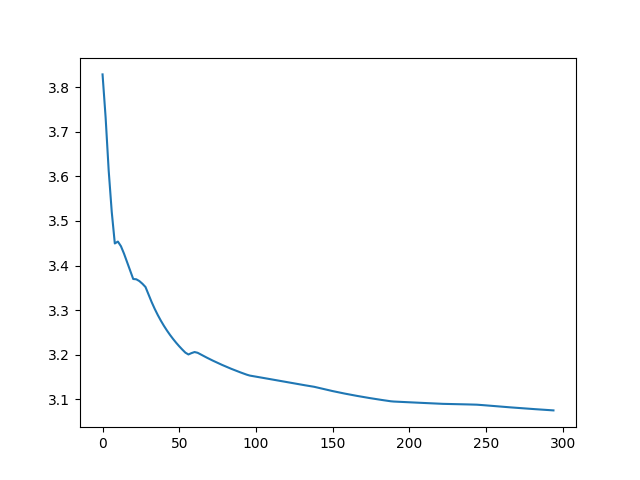
\includegraphics[scale=0.5]{beta_2n1}\label{fig:beta2n1}

On observe bel et bien le petit saut en $n = 62$
cependant... on observe deux pics avant cela, un pic en $n = 14$ et un faux pic en $n = 24$ qui en réalité ne casse pas la conjecture. Mais ce qui est important, c'est qu'on observe une exception bien avant $n = 62$! or pour $n = 14$ on peut aisément faire le calcul avec l'algorithme de brute force. Et l'algorithme de brute force et segment coïncident pour $n \leq 17$
On alors bien que la conjecture était fausse. On pourrait alors imaginer de nouvelles conjectures, en particulier sur où sont les exceptions. Il a d'abord été proposé par mon encadrant des formules basées sur $4^n$ car 4 est un maximum, 16 est proche d'une exception et 64 est un maximum local. Cependant, n'ayant aucune autre exception pour $n \leq 300$ la série se casse. Peut être peut on alors se dire qu'il s'agissait d'exceptions et qu'il n'y en a plus après, et pourtant...

  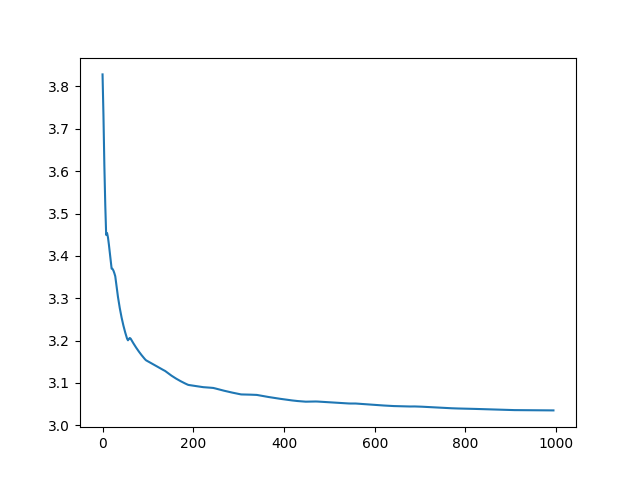
\includegraphics[scale=0.5]{beta_2n2}\label{fig:beta2n2}

On observe rien de plus sur cette figure, elle semble lisse après les exceptions et prend désormais en compte les $n \leq 1000$ ce qui va bien plus loin, mais.. en cherchant avec python des maximums et des minimums, voici ce que l'on obtient:

\begin{verbatim}
local maximum:  4
local minimum:  12
local maximum:  14
local minimum:  60
local maximum:  64
local minimum:  450
local maximum:  474
local maximum:  476
local minimum:  550
local maximum:  560
local minimum:  678
local maximum:  688
local minimum:  802
local minimum:  804
local maximum:  806
\end{verbatim}

On observe nos anciens pics mais on observe surtout de nouveaux pics qui ont l'air complètement chaotiques. Cet air chaotique est probablement donné par des solutions d'équations trigonométrique mais cela montre surtout qu'il n'y a pas d'espoir de trouver des solutions simples, que nos conjectures sont justes fausses et donc que ce que certains chercheurs pensaient vrai ne pouvaient l'être... Voici quelque part ma contribution dans le domaine des conjectures. Et tout cela grâce à des algorithmes optimisés comme possible.
	
	\section{Conclusion}

Dans ce rapport, nous aurons alors pu obtenir un résultat en apparence mineur sur la série des alpha mais nous aurons également pu voir que des conjectures pourtant considérées comme étant vraies sont en réalité bien fausses rendant ainsi les conjectures précieuses et les petits résultats importants. Malgré tout, il faut continuer d'espérer que les grandes conjectures soient correctes et espérer pouvoir résoudre ces questions ouvertes telles que:

\begin{itemize}

\item $\alpha_4$ est maximum strict?
\item $\alpha_{2^n}$ décroissante?
\item Pire configuration convexe et donc uniforme (cas paire)?
\item Résolution du cas convexe P? NP-dur?
\item Résolution du cas uniforme dans P?

J'ai pu également trouver une borne correcte pour $\alpha_6$ dans le cas où les points sont dans le cas convexe en suivant la même méthode que pour $\alpha_5$ cependant je n'ai pas réussi à généraliser. Une borne de $\alpha_6$ reste alors un travail possible.

\end{itemize}
	
	\section{Annexe}
	
	\input{Contexte_social_institutionnel.tex}
	
	\subsection{ressources du stage}
	
	\href{https://github.com/lum33n/freeze-tag-internship/tree/main}{Git}

\end{document}